\documentclass[multi=false, tikz, border=2mm]{article}
\usepackage[siunitx]{circuitikz}
\usepackage{graphicx}
\usepackage{float}
\usepackage[center]{caption}
\usepackage{amsmath}
\usepackage{mathptmx}
\usepackage{tikz}
\usepackage[colorlinks=true, allcolors=blue, unicode]{hyperref}
\usetikzlibrary{arrows, decorations.markings}
\usepackage[romanian]{babel}
\usepackage[export]{adjustbox}
\usepackage[skins, theorems]{tcolorbox}
\tcbset{highlight math style = {enhanced, colframe=red, colback=white, arc=0pt, boxrule=1pt}}
\newcommand\tab[1][0.6cm]{\hspace*{#1}}
\usepackage{fancyhdr}
\renewcommand{\headrulewidth}{2pt}
\renewcommand{\footrulewidth}{1pt}
\usepackage{listings}
\usepackage{color} %red, green, blue, yellow, cyan, magenta, black, white
\definecolor{mygreen}{RGB}{28,172,0} % color values Red, Green, Blue
\definecolor{mylilas}{RGB}{170,55,241}
\pagestyle{fancy}
\title{TEM\u{a} ELTH}
\author{Petruc Rares}
\fancyhf{}
\rhead{Petruc Rare\c{s}}
\lhead{TEM\u{A} ELTH}
\rfoot{Pagina \thepage}

\begin{document}

\lstset{language=Matlab,%
	%basicstyle=\color{red},
	breaklines=true,%
	morekeywords={matlab2tikz},
	keywordstyle=\color{blue},%
	morekeywords=[2]{1}, keywordstyle=[2]{\color{black}},
	identifierstyle=\color{black},%
	stringstyle=\color{mylilas},
	commentstyle=\color{mygreen},%
	showstringspaces=false,%without this there will be a symbol in the places where there is a space
	numbers=left,%
	numberstyle={\tiny \color{black}},% size of the numbers
	numbersep=9pt, % this defines how far the numbers are from the text
	emph=[1]{for,end,break},emphstyle=[1]\color{red}, %some words to emphasise
	%emph=[2]{word1,word2}, emphstyle=[2]{style},    
}

\thispagestyle{plain}
\begin{center}

	\Large
	\textbf{TEM\u{A}}
		
	\vspace{0.4cm}
	\large
	-Electrotehnic\u{a}-
	
	\vspace{4cm}

\end{center}


\vspace{0.9cm}
\textbf{Abstract} Documentul de mai jos reprezint\u{a} tema mea la Electrotehnic\u{a}, tem\u{a} pe care am efecutat-o de-a lungul a opt zile, cu un timp de lucru mediu de 5-6 ore pe zi. Am urm\u{a}rit \^{i}ndeaproape metodele prezentate \^{i}n breviarul de seminar pus la dispozi\c{t}ie pe acs.curs, cu ajutorul c\u{a}rora am rezolvat cerin\c{t}ele propuse \^{i}n tem\u{a}.



Cu mult ajutor de pe paginile Overleaf, Stack Exchange, dar mai ales din arhiva pus\u{a} la dispozi\c{t}ie pe pagina de acs.curs (Template latex v4), sper c\u{a} am reu\c{s}it s\u{a} duc, cu succes, tema la bun sf\^{a}r\c{s}it \c{s}i s\u{a}-i ofer un aspect c\^{a}t se poate de pl\u{a}cut.\\


\vspace{4cm}

\noindent
\makebox[\textwidth][r]{
	\begin{minipage}{0.5\textwidth}
	Petruc Rare\c{s}\\
	Grupa 312CD\\
	Facultatea de Automatic\u{a} \c{s}i Calculatoare\\
	Universitatea POLITEHNICA din Bucure\c{s}ti\\
	03.05.2020\\
\end{minipage}
}

\renewcommand\tablename{Tabelul}
\date{\today}  % sau puneti data explicit - va ramane fixata
\pagebreak
	
	% aici am modificat contentsname default
	% in "Cuprins"
	
	\renewcommand*\contentsname{Cuprins}
	
	\tableofcontents
	
	\pagebreak
	
	\section{Generarea unui circuit}
		\label{task1}
		
		\tab {\color{purple}{\bf Primul pas}} \^{i}n generarea circuitului electric cu solu\c{t}ii \^{i}ntregi a fost construirea unei perechi de grafuri, unul de curen\c{t}i \c{s}i unul de tensiuni \c{s}i a unui arbore, dup\u{a} care m-am ghidat \^{i}n a pune curen\c{t}i pe ramurile sale \c{s}i tensiuni pe coarde.
		
	
	\begin{figure}[H]	
	\begin{minipage}{0.5\textwidth}
			\centering	
			\begin{circuitikz}[american]
				\draw(0, 0) to [short, i = -1<\ampere>, *-*] (4, 0);
				\draw(4, 0) to (4, -4);
				\draw(4, -4) to [short, i = 6<\ampere>, *-*](0, -4);
				\draw(0, -4) to (0, 0);
				\draw(0, -4) -- (1, -3) to [short, i = 3<\ampere>] (3, -1) to (4, 0);
				\draw(0, -4) -- (0, -6) to (4, -6) to (4, -4);
				;
			\end{circuitikz}
	\end{minipage}
	\begin{minipage}{0.5\textwidth}
			\centering		
			\begin{circuitikz}[american]
				\tikzset{myptr/.style={decoration={markings, mark=at position 1 with {\arrow[scale=3, >=stealth]{>}}},
						postaction={decorate}}}
				\draw [myptr, *-*](0, 0) -- (0, 4) node[midway, left] {\SI{-1}{\volt}};
				\draw [myptr](0, 4) -- (4, 4);
				\draw [myptr](4, 4) -- (4, 0) node[midway, right] {{\SI{-2}{\volt}}};
				\draw [myptr](4, 0) -- (0, 0);
				\draw [myptr](0, 0) --(4, 4);
				\draw [myptr]node[left] {A}(0, 0) -- (0, -2) -- (4, -2) node[midway, above] {{\SI{-6}{\volt}}} -- (4, 0) ;	
			\end{circuitikz}
	\end{minipage}
% \u{a}
% \^{a}
% \^{i}
%\c{s}
% \c{t}
	\caption{Grafurile ini\c{t}iale: st\^{a}nga - graful de curen\c{t}i; dreapta - graful de tensiuni.}
	\label{fig:grafuri_initial}
	\end{figure}

	 {\color{purple}{\bf Al doilea pas}} \^{i}n generarea circuitului a fost s\u{a} completez grafurile \c{s}i s\u{a} verific corectitudinea complet\u{a}rii cu ajutorul teoremei lui Tellegen.
	 
	\begin{figure}[H]
	\begin{minipage}{0.5\textwidth}
		\centering	
		\begin{circuitikz}[american]
			\draw(0, 0) to [short, i = -1<\ampere>, *-*] (4, 0);
			\draw(4, 0) to [short, i = 2<\ampere>, red](4, -4);
			\draw(4, -4) to [short, i = 6<\ampere>, *-*](0, -4);
			\draw(0, -4) to [short, i = -1<\ampere>, red](0, 0);
			\draw(0, -4) -- (1, -3) to [short, i = 3<\ampere>] (3, -1) to (4, 0);
			\draw(0, -4) -- (0, -6) to [short, i = 4<\ampere>, red] (4, -6) to (4, -4);
			;
		\end{circuitikz}
	\end{minipage}
	\begin{minipage}{0.5\textwidth}
		\centering		
		\begin{circuitikz}[american]
			\tikzset{myptr/.style={decoration={markings, mark=at position 1 with {\arrow[scale=3, >=stealth]{>}}},
					postaction={decorate}}}
			\draw [myptr, *-*](0, 0) -- (0, 4) node[midway, left] {\SI{-1}{\volt}};
			\draw [myptr](0, 4) -- (4, 4) node[midway, above, red] {\SI{-3}{\volt}};
			\draw [myptr](4, 4) -- (4, 0) node[midway, right] {{\SI{-2}{\volt}}};
			\draw [myptr](4, 0) -- (0, 0) node[midway, above, red] {\SI{6}{\volt}};
			\draw [myptr](0, 0) --(4, 4) node[midway, left, red] {\SI{-4}{\volt}};
			\draw [myptr]node[left] {A}(0, 0) -- (0, -2) -- (4, -2) node[midway, above] {{\SI{-6}{\volt}}} -- (4, 0) ;	
		\end{circuitikz}		
	\end{minipage}
	\caption{Solu\c{t}ia circuitului generat: st\^{a}nga - graful de curen\c{t}i; dreapta - graful de tensiuni.}
	\label{fig:grafuri_final}
	\end{figure}
	\pagebreak
	
	\begin{equation} \label{eq: Orice}
	\tcbhighmath[colframe=blue, drop fuzzy shadow = green]{
	\begin{aligned}
	P_{R} &= (-1)\cdot(-1) + (6)\cdot6 + 3\cdot(-4) + (4)\cdot(-6) + (-1)\cdot(-3) + 2\cdot(-2) = 0 W,\\
	P_{G} &= 0 W.
	\end{aligned}}
	\end{equation}
	
	Rela\c{t}iile din \ref{eq: Orice} valideaz\u{a} corectitudinea valorilor curen\c{t}ilor \c{s}i tensiunilor, fapt pentru care putem trece la {\color{purple}{\bf pasul 3}}, \^{i}n care complet\u{a}m laturile cu elementele cerute \^{i}n cadrul cerin\c{t}ei, \c{s}i stabilim \c{s}i o serie de valori convenabile.
	
	\begin{figure}[H]
			\centering
		\begin{circuitikz}[american]	
			\draw(0, 0) to [R, l = 1<\ohm>, *-*](0,4) % R1
			 (2, 4) to [V, l_ = 2<\volt>] (0, 4) % V2
			 (2, 4) to [R, l = 1<\ohm>] (4, 4) % R2
			 (4, 4) to [I, l = 2<\ampere>, *-*] (4, 0) % J1
			 (4, 0)to [R, l=1<\ohm>] (0, 0) % R3
			 %(0, 0) to [V, l_=1<\volt>](2, 0) % V3
			(0, 0) -- (0, -2) to [I, l_=4<\ampere>](4, -2) -- (4, 0) % J2
			
			(4, 4) -- (3, 3) to [V, l = 4<\volt>] (1, 1) -- (0, 0) %V2	
		;
		\end{circuitikz}
		\caption{Circuit.}\label{fig: circuit}
		\end{figure}
	
	Din fig. \ref{fig: circuit}, reies urm\u{a}toarele caracteristici topologice ale circuitului:
	
	\begin{table}[h]
	\caption{Topologia circuitului.}\label{tab: tab_top}
	\begin{center}
	\begin{tabular}{|c|}	
			\hline
			Topologie\\			
			\hline
			L = 6\\
			\hline
			N = 4\\
			\hline
			$n_{SIC}$ = 2\\
			\hline
			$n_{SIT}$ = 1\\
			\hline
	\end{tabular}
	\end{center}
	\end{table}

	\pagebreak
		
	\section{Metode sistematice eficiente}
	\tab \^{I}n cadrul acestui task, am analizat care ar fi cea mai eficient\u{a} metod\u{a} pentru rezolvarea circuitului generat in fig. {\ref{fig: circuit}} \c{s}i, conform acesteia, am rezolvat circuitul.
	\vspace{-0.4cm}
	\subsection{Tabel metode}
	\tab Din tabelul \ref{tab: tab_top} reies urm\u{a}toarele date:
	\vspace{-0.2cm}
	\begin{table}[h]
	\begin{center}	
	\caption{Tabel metode.}\label{tab_metode}
	\begin{tabular}{|p{10cm}|l|}		
			\hline
			Metoda & Num\u{a}r de ecua\c{t}ii\\
			\hline
			\hline
			Kirchoff clasic & 2L = 12\\
			\hline
			Kirchoff in curen\c{t}i & L $-$ N $+$ 1 $=$ 3\\
			\hline
			Kirchoff in tensiuni & N $-$ 1 = 3\\
			\hline
			Curen\c{t}i de coarde (curen\c{t}i de bucle/curen\c{t}i ciclici) & L $-$ N $+$ 1 $-$ $n_{SIC}$ = 1\\
			\hline
			Tensiuni \^{i}n ramuri(po\c{t}entiale ale nodurilor dac\u{a} SIT formeaz\u{a} un subgraf conex) & N $-$ 1 $-$ $n_{SIT}$ = 2\\
			\hline
	\end{tabular}
	\end{center}
	\end{table}
		
\vspace{-0.9cm}
	\subsection{Rezolvarea circuitului cu metoda cea mai eficient\u{a}}
	\tab Observ\u{a}m din tabelul \ref{tab_metode} c\u{a} vom ob\c{t}ine cel mai mic num\u{a}r de ecua\c{t}ii pentru metoda curen\c{t}ilor de coarde, motiv pentru care, mai departe, vom lucra cu aceasta.\\
	\tab Marchez cu ro\c{s}u arborele normal \c{s}i generez bucla [1], bucl\u{a} generat\u{a} de coarda ce nu con\c{t}ine SIC.
	
	\begin{figure}[H]\centering
	\begin{circuitikz}[american]
		
		\draw(0, 0) to [R, l = 1<\ohm>, *-*, i = ${I}$](0,4) % R1
		(2, 4) to [V, l_ = 2<\volt>, i = ${I}$] (0, 4) % V2
		(2, 4) to [R, l = 1<\ohm>] (4, 4) % R2;
		(4, 4) to [I, l = 2<\ampere>, *-*, i = ${2A}$] (4, 0) % J1
		(4, 0)to [R, l=1<\ohm>, i = ${6A}$] (0, 0) % R3
		%(0, 0) to [V, l_=1<\volt>](2, 0) % V3
		(0, 0) -- (0, -2) to [I, l_=4<\ampere>, *-*, i = ${4A}$](4, -2) -- (4, 0) % J2
		(4, 4) -- (3, 3) to [V, l = 4<\volt>, i = ${2A-I}$] (1, 1) -- (0, 0) %V2	
		;
		
		% reprezentarea arborelui normal:
						
		\draw[red, line width = 0.5mm](4, 4) -- (0, 4) (4, 4) -- (0, 0) (0, 0) -- (4, 0);

		% reprezentarea buclelor:
		\draw[green] (0.8, 2) to [short, i = ${[1]}$](0.8, 3) -- (1.5, 3) -- (0.8, 2);
		
	\end{circuitikz}
	\caption{Circuit + arbore normal.}\label{fig: rezolvare_circuit}
	\end{figure}

	\begin{center}
		
	Scriem Kirchoff II pentru bucla independent\u{a} aleas\u{a} la pasul anterior:
	\begin{equation} \label{eq: ec1}
		[1]: 1\cdot{I} + 1\cdot{I} = 2 - 4,
	\end{equation}
			
	 din \ref{eq: ec1} reiese banal c\u{a}:
	 \begin{equation} \label{eq: ec2}
 		2\cdot{I} = -2 => I = {\SI{-1}{\ampere}}.
	\end{equation}
	\end{center}		
		
	\tab Acum putem completa grafurile de curen\c{t}i \c{s}i tensiuni (Fig. \ref{fig: gdc} \c{s}i Fig. \ref{fig: gdu}), \c{s}i observ\u{a}m c\u{a} sunt identice cu grafurile generate \^{i}n Fig. \ref{fig:grafuri_final}:
		
		
	\begin{minipage}{0.5\textwidth}
	\begin{figure}[H]
	\centering	
	\begin{circuitikz}[american]
		\draw(0, 0) to [short, i = -1<\ampere>, *-*] (4, 0);
		\draw(4, 0) to [short, i = 2<\ampere>](4, -4);
		\draw(4, -4) to [short, i = 6<\ampere>, *-*](0, -4);
		\draw(0, -4) to [short, i = -1<\ampere>](0, 0);
		\draw(0, -4) -- (1, -3) to [short, i = 3<\ampere>] (3, -1) to (4, 0);
		\draw(0, -4) -- (0, -6) to [short, i = 4<\ampere>] (4, -6) to (4, -4);
		;
	\end{circuitikz}
	\caption{Graful de curen\c{t}i.}\label{fig: gdc}
	\end{figure}
	\end{minipage}
	\begin{minipage}{0.5\textwidth}
	\begin{figure}[H]
	\centering		
	\begin{circuitikz}[american]
	\tikzset{myptr/.style={decoration={markings, mark=at position 1 with {\arrow[scale=3, >=stealth]{>}}},
			postaction={decorate}}}
		\draw [myptr, *-*](0, 0) -- (0, 4) node[midway, left] {\SI{-1}{\volt}};
		\draw [myptr](0, 4) -- (4, 4) node[midway, above] {\SI{-3}{\volt}};
		\draw [myptr](4, 4) -- (4, 0) node[midway, right] {{\SI{-2}{\volt}}};
		\draw [myptr](4, 0) -- (0, 0) node[midway, above] {\SI{6}{\volt}};
		\draw [myptr](0, 0) --(4, 4) node[midway, left] {\SI{-4}{\volt}};
		\draw [myptr]node[left] {A}(0, 0) -- (0, -2) -- (4, -2) node[midway, above] {{\SI{-6}{\volt}}} -- (4, 0) ;	
	\end{circuitikz}		
	\caption{Graful de tensiuni.}\label{fig: gdu}
	\end{figure}
	\end{minipage}

	\pagebreak
	\section{Generatorul echivalent de tensiune}
	\vspace{-.25cm}
	\subsection{Echivalarea circuitului fa\c{t}\u{a} de bornele A \c{s}i B}
	\begin{samepage}
	\begin{figure}[H]
	\centering

	% TOT CE ESTE PUS DUPA '%' LA FINAL DE RAND REPEZINT\u{a}
	% ELEMENTUL CORESPUNZATOR LINIEI IN LTSPICE	
		
	\begin{circuitikz}[american]
			
		\draw (2, 4) to [V, l_ = 2<\volt>, -*] node[above = 0.1cm]{B}(0, 4) % V2
		(2, 4) to [R, l = 1<\ohm>] (4, 4) % R2
		(4, 4) to [I, l = 2<\ampere>, *-*] (4, 0) % J1
		(4, 0)to [R, l=1<\ohm>, *-*] (0, 0) % R3
		node[below left= 0.01cm]{A}(0, 0) -- (0, -2) to [I, l_=4<\ampere>](4, -2) -- (4, 0) % J2
		
		(4, 4) -- (3, 3) to [V, l = 4<\volt>] (1, 1) -- (0, 0) %V2	
		;
		
		\node (A) at (0,0){};
		\node (B) at (0,4){}
		edge [<-, thick, bend right, red] node [pos=0.5, left] {$U_{AB0}$} (A) ;
		
	\end{circuitikz}
	\vspace{-0.2cm}
	\caption{Circuitul activ, \^{i}n gol.}\label{fig: Thevenin}
	\end{figure}
	\vspace{-0.3cm}
	\tab Am ales rezistorul dintre punctele A \c{s}i B drept rezistor de sarcin\u{a}. Mai int\^{a}i desen\u{a}m circuitul \^{i}n gol \c{s}i marc\u{a}m sensul de referin\c{t}\u{a} al tensiunii de calculat (Fig. \ref{fig: Thevenin}), complet\u{a}m grafurile de curent (Fig. \ref{fig: gdc2}) \c{s}i tensiune (Fig. \ref{fig: gdu2}), cu ra\c{t}ionamente simple:
	\vspace{-0.2cm}
	
	\vspace{-0.4cm}
	
	\begin{minipage}{0.49\textwidth}
	\begin{figure}[H]
	\centering	
	\begin{circuitikz}[american]
				
		\draw(0, 0) to [short, i = 0<\ampere>, *-*] (4, 0);
		\draw(4, 0) to [short, i = 2<\ampere>](4, -4);
		\draw(4, -4) to [short, i = 6<\ampere>, *-*](0, -4);
		\draw(0, -4) -- (1, -3) to [short, i = 2<\ampere>] (3, -1) to (4, 0);
		\draw(0, -4) -- (0, -6) to [short, i = 4<\ampere>] (4, -6) to (4, -4);
				
	\end{circuitikz}
	\caption{Graful de curen\c{t}i al circuitului activ, \^{i}n gol.}\label{fig: gdc2}
	\end{figure}
	\end{minipage}
	\begin{minipage}{0.49\textwidth}
	\begin{figure}[H]
	\centering		
	\begin{circuitikz}[american]
	\tikzset{myptr/.style={decoration={markings, mark=at position 1 with {\arrow[scale=3, >=stealth]{>}}},
			postaction={decorate}}}

		\node (A) at (0,0){};
		\node (B) at (0,4){}
		edge [<-, thick, bend right, red] node [pos=0.5, left] {$U_{AB0}$} (A) ;
		\draw [myptr, *-*]node[above = 4cm]{B}(0, 4) -- (4, 4) node[midway, above] {\SI{-2}{\volt}};
		\draw [myptr](4, 4) -- (4, 0) node[midway, right] {{\SI{-2}{\volt}}};
		\draw [myptr, *-*](4, 0) -- (0, 0) node[midway, above] {\SI{6}{\volt}};
		\draw [myptr](0, 0) --(4, 4) node[midway, left] {\SI{-4}{\volt}};
		\draw [myptr]node[left] {A}(0, 0) -- (0, -2) -- (4, -2) node[midway, above] {{\SI{-6}{\volt}}} -- (4, 0) ;
		
	\end{circuitikz}
	\caption{Graful de tensiuni al circuitului activ, \^{i}n gol.}\label{fig: gdu2}
	\end{figure}
	\end{minipage}
	\end{samepage}
	\vspace{-0.4cm}
	Reiese imediat din Fig.\ref{fig: gdu2} c\u{a}:

	\vspace{-0.1cm}
	\begin{equation} \label{eq: UAB0}
	{U_{AB0}} = -4 - (-2) ={\SI{-2}{\V}},
	\end{equation}
		
	Calculul rezisten\c{t}ei circuitului pasivizat \c{s}i \^{i}n gol; Desen\u{a}m acum schema circuitului pasivizat \c{s}i \^{i}n gol:
	
	\begin{figure}[H]\centering
	\begin{circuitikz}[american]

		\draw(0, 4) to [R, l = 1<\ohm>] (4, 4) % R2;
		(4, 4) to (4, 3) (4, 1) to (4, 0) % J1
		(4, 0)to [R, l=1<\ohm>] (0, 0) % R3
		%(0, 0) to [V, l_=1<\volt>](2, 0) % V3
		(0, 0) -- (0, -2) to (1, -2) (3, -2) to (4, -2) -- (4, 0) % J2
		
		(4, 4) -- (3, 3) to (1, 1) -- (0, 0) %V2	
		;
			
	\tikzset{myptr/.style={decoration={markings, mark=at position 1 with {\arrow[scale=1, >=stealth]{>}}},
			postaction={decorate}}}					
			
	\draw[myptr, red](-0.5, 2) to node[midway, above] {$R_{AB0}$} (0.3, 2);
	\end{circuitikz}
	\caption{Circuitul pasiv, in gol.}\label{fig: circ_pasiv}		
	\end{figure}
		
	Cum topologia circuitului este de tip serie-paralel, rezisten\c{t}a echivalent\u{a} se ob\c{t}ine imediat: 
	\begin{equation} \label{eq: RAB0}
		{R_{AB0}} = {\SI{1}{\ohm}},
	\end{equation}
		
	Conform formulei Thévenin rezult\u{a}:

	\begin{equation} \label{eq: IAB}
		{I_{AB}} = \frac{U_{AB0}}{{R_{AB0}} + {R_{AB}}} = \frac{-2}{1+1} = {\SI{-1}{\ampere}}.
	\end{equation}		
			
	\begin{figure}[H]\centering	
	\begin{circuitikz}[american]
				
		\draw (0, 0) to [R, l = 1<\ohm>](0, 2)
		(0, 2) to [V, l = 2<\volt>] (0, 4) 
		(0, 4) -- (3, 4)
		(3, 4) to [R, l = 1<\ohm>] (3, 0)
		(3, 0) -- (0, 0);

	\end{circuitikz}			
	\caption{Schema generatorului echivalent.}\label{fig: echivThev}		
	\end{figure}	
		
	\pagebreak
	
\begin{figure}[h!b]
\begin{center}
	%\hspace*{-1cm}
%	trim=100 75 100 100,clip,width=\textwidth
	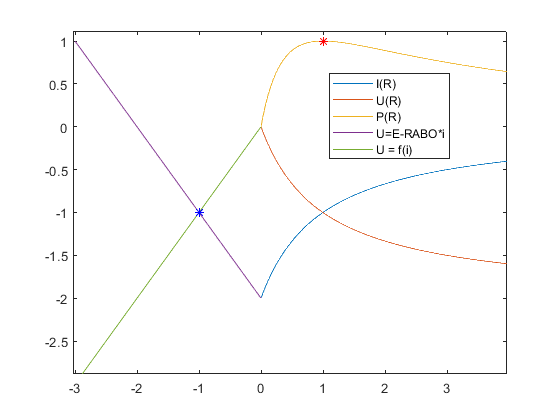
\includegraphics[clip, width=\textwidth]{ELTH_GRAFICE}.
\end{center}
\vspace{-1.1cm}
\caption{Reprezentarea graficelor.}\label{fig:grafice}
\end{figure}

Observ\u{a}m \^{i}n Fig. \ref{fig:grafice} marcat cu o stelu\c{t}\u{a} ro\c{s}ie punctul de coordonate (1, 1) (\si{\ohm}, \si{\watt}), punct corespunz\u{a}tor totodata perechii de valori: rezisten\c{t}a ini\c{t}ial\u{a}, valoarea puterii pentru rezisten\c{t}a ini\c{t}ial\u{a}, c\^{a}t \c{s}i perechii de valori: rezisten\c{t}a pentru care puterea e maxim\u{a} \c{s}i implicit valoarea acesteia.

Ne a\c{s}teptam s\u{a} se intample acest lucru, dup\u{a} cum putem vedea \c{s}i \^{i}n Fig. \ref{fig:ValoriPR}, unde $R_{AB}$ este egal cu rezisten\c{t}a ini\c{t}ial\u{a} \c{s}i $R_{ab}$ cu rezisten\c{t}a pentru care puterea este maxim\u{a}, pentru c\u{a} \c{s}tim c\u{a} puterea este maxim\u{a} atunci c\^{a}nd rezisten\c{t}a de sarcin\u{a}, $R_{AB}$ este egal\u{a} cu rezisten\c{t}a echivalent\u{a} a re\c{t}elei pasivizate ($R_{AB0}$).

\begin{figure}[h!b]
	\begin{center}
		\hspace*{-3cm}
		%	trim=100 75 100 100,clip,width=\textwidth
		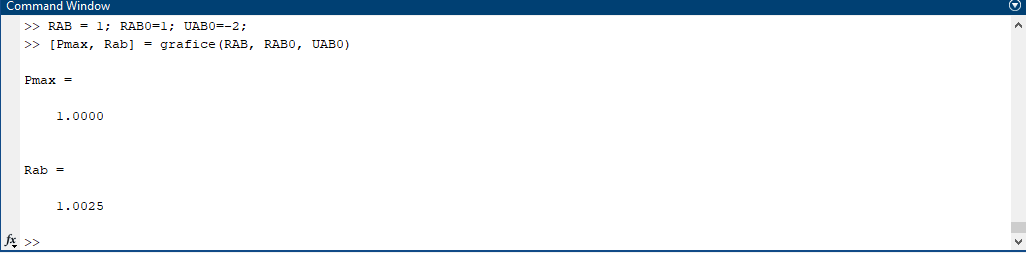
\includegraphics[clip, width=180mm]{ValoriPutereRezistenta}.
	\end{center}
	\caption{Valori ob\c{t}inute pentru Pmax si rezisten\c{t}a asociat\u{a}.}\label{fig:ValoriPR}
\end{figure}

\subsection{Punctul static de func\c{t}ionare pentru rezistorul liniar \c{s}i generatorul echivalent} \label{sssec: PSF1}
	\tab Am reprezentat pe acela\c{s}i grafic din Fig. \ref{fig:grafice} o stelu\c{t}\u{a} de culoare albastr\u{a}, ce reprezint\u{a} punctul static de func\c{t}ionare aflat la intersec\c{t}ia dreptei de sarcin\u{a} (dreapta marcat\u{a} cu mov) cu caracteristica liniar\u{a} a tensiunii la bornele rezistorului $R_{AB}$(dreapta marcat\u{a} cu verde), av\^{a}nd coordonatele (-1, -1) (\si{\ohm}, \si{\watt}).
	
\subsection{Punctul static de func\c{t}ionare pentru dioda semiconductoare \c{s}i generatorul echivalent} \label{sssec: PSF2}

	\tab Am ales $I_{S}$ de ordinul pA si $V_{T}$ de ordinul mV.	
	Ca metoda numeric\u{a}, am lucrat cu metoda bisec\c{t}iei pentru c\u{a} este mai robust\u{a} \c{s}i dup\u{a} cum reise din graficele din Fig. \ref{fig:Depiu1} sau Fig. \ref{fig:Depiu2}, aveam posibilitatea ca \^{i}n urma aplic\u{a}rii metodei tangentei sau secantei s\u{a} ajung pe o por\c{t}iune unde aveam derivata 0, iar ca urmare, algoritmul divergea.
	Vreau s\u{a} men\c{t}in aceeasi dreapt\u{a} de sarcin\u{a} in cazul celor dou\u{a} grafice, unde dreapta de sarcina are formula: 
	\begin{equation} \label{eq:ecTaieturi}
	i(u) = \frac{U_{ABO}}{R_{AB0}}-\frac{u}{R_{AB0}}
	\end{equation}
	Liniile 14 at\^{a}t din Fig. \ref{fig:ValDirecta}, c\^{a}t \c{s}i din Fig. \ref{fig:ValInversa}, reprezint\u{a} valoarea oric\u{a}rei din caracteristici (a diodei sau a generatorului echivalent) in punctul r.
	Vom avea 2 cazuri:
	
	{\color{orange}{\bf Cazul 1}} (Polarizare direct\u{a}):
	
	\begin{equation} \label{eq:ecPolDir}
	i(u) = I_{S}(e^{\frac{u}{V_{T}}}-1)
	\end{equation}
	
	
	\begin{figure}[H]
	\hspace{1.7cm}
	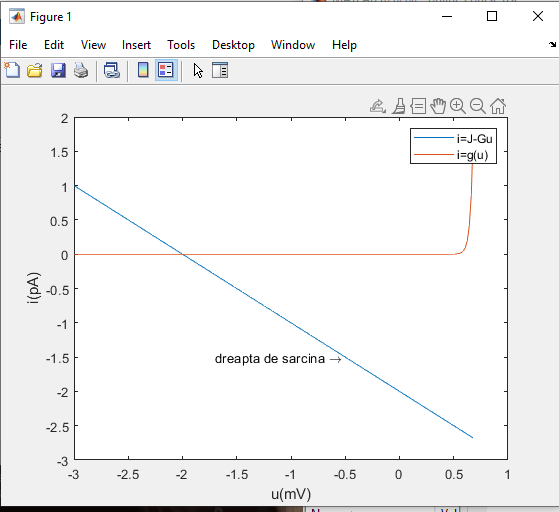
\includegraphics[trim = 20 0 23 70, clip, scale=0.6]{PolarizareDirecta}
	\caption{Dependen\c{t}a i functie de u (polarizare direct\u{a}).}\label{fig:Depiu1}
	\end{figure}
	
	 Observ\u{a}m c\u{a} valoarea PSF se inv\^{a}rte in jurul valorii de (-2, 0) (V, A), deci avem grij\u{a} ca intervalul pentru codul metodei bisec\c{t}iei, din Fig. \ref{fig: CodBisectie} s\u{a} contin\u{a} pe "-2". 
	
	\begin{figure}[H]
		\hspace{.6cm}
		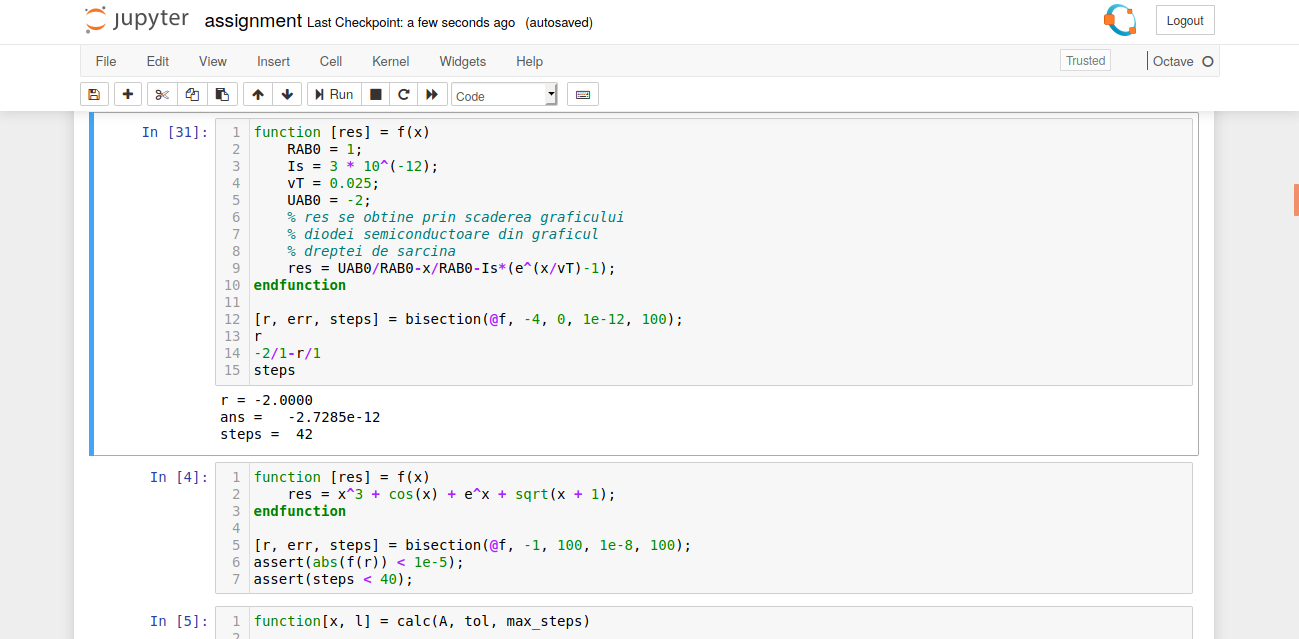
\includegraphics[trim = 200 180 610 110, clip, scale=0.6]{PozaValPolDirecta}
		\caption{Valori ob\c{t}inute \^{i}n urma rul\u{a}rii codului pentru cazul de polarizare direct\u{a}.}\label{fig:ValDirecta}
	\end{figure}
\vspace{-0.4cm}
Observ\u{a}m din Fig. \ref{fig:ValDirecta} c\u{a} \^{i}n urma rul\u{a}rii codului, ob\c{t}inem valorile la care ne a\c{s}tept\u{a}m dupa numai 42 de pa\c{s}i.
\pagebreak

	{\color{orange}{\bf Cazul 2}} (Polarizare invers\u{a}):
	\begin{equation} \label{eq:ecPolInv}
	i(u) = I_{S}(1-e^{\frac{-u}{V_{T}}})
	\end{equation}
	\vspace{-0.6cm}
	\begin{figure}[H]
		\hspace{1.7cm}
		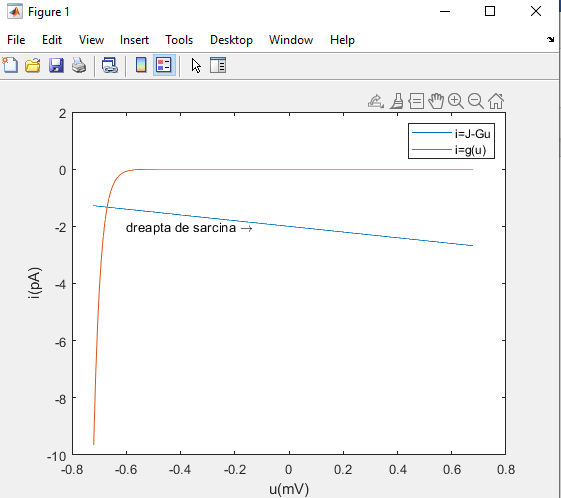
\includegraphics[trim = 20 0 23 70, clip, scale=0.6]{PolarizareInversa}
		\caption{Depende i func\c{t}ie de u (polarizare invers\u{a}).}\label{fig:Depiu2}
	\end{figure}

	\vspace{-0.3cm}
	Observ\u{a}m c\u{a} valoarea PSF se \^{i}nv\^{a}rte in jurul valorii de (-0.7, -1) (V, A), deci avem grij\u{a} ca intervalul pentru codul metodei bisec\c{t}iei, din Fig. \ref{fig: CodBisectie} s\u{a} con\c{t}in\u{a} "-0.7". 

	\begin{figure}[H]
	\hspace{.6cm}
	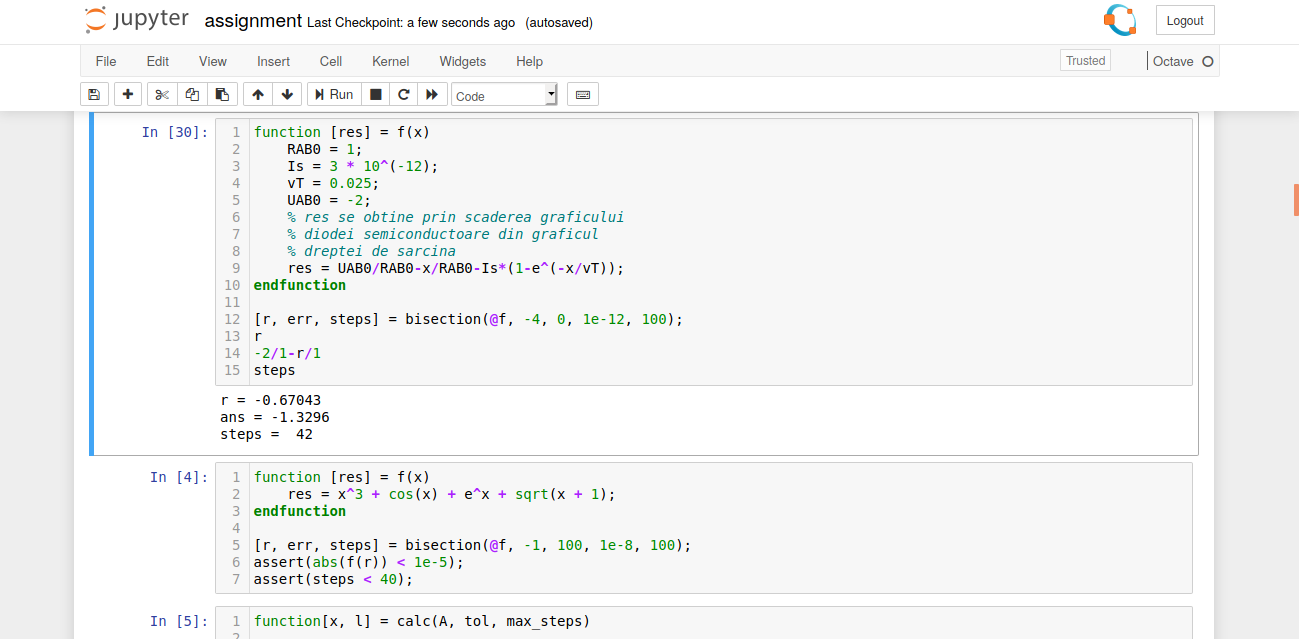
\includegraphics[trim = 200 180 610 110, clip, scale=0.6]{PozaValPolInversa}
	\caption{Valori ob\c{t}inute \^{i}n urma rul\u{a}rii codului pentru cazul de polarizare invers\u{a}.}\label{fig:ValInversa}
\end{figure}

\vspace{-0.3cm}
Observ\u{a}m din Fig. \ref{fig:ValInversa} c\u{a} in urma rul\u{a}rii codului, ob\c{t}inem valorile la care ne a\c{s}tept\u{a}m numai dupa 42 de pa\c{s}i.

\pagebreak	
	
	\section{Surse comandate}
	\vspace{-0.2cm}
	\^{I}n cadrul acestei cerin\c{t}e, am avut de generat dou\u{a} circuite diferite, av\^{a}nd o SUCI, respectiv o SICU \c{s}i de a le simula in LTSPICE. Ata\c{s}ez netlistul figurilor \ref{fig:SIT_TO_SUCI} \c{s}i \ref{fig: SIC_TO_SICU} in \ref{fig: NETLISTS}. % nu mai scriu Fig.?
	\vspace{-0.6cm}
	\subsection{Transformare SIT \^{i}n SUCI}
	
	\vspace{-0.8cm}
	\begin{figure}[H]
	\centering	
	\begin{circuitikz}[american]
				
		\draw(0, 0) to [R, l = 1<\ohm>, *-*](0,4) % R1
		(2, 4) to [cV, l_ = -$\frac{1}{3}I$, color=red, red] (0, 4) % V2
		(2, 4) to [R, l = 1<\ohm>] (4, 4) % R2
		(4, 4) to [I, l = 2<\ampere>, *-*] (4, 0) % J1
		(4, 0) -- (3, 0)
		(3, 0)to [R, l=1<\ohm>] (1, 0) % R3
		(1, 0) to [short, i = $I$, red](0, 0)
		(0, 0) -- (0, -2) to [I, l_=4<\ampere>](4, -2) -- (4, 0) % J2
		
		(4, 4) -- (3, 3) to [V, l = 4<\volt>] (1, 1) -- (0, 0) %V2	
		;
		
	\end{circuitikz}
\vspace{-0.2cm}
	\caption{Circuit generat prin \^{i}nlocuirea SIT cu SUCI.}\label{fig: SUCI}
	\vspace{-0.3cm}
	\begin{flushleft}
	\tab Rezisten\c{t}a de transfer este egal\u{a} cu -$\frac{1}{3}$, iar din Fig. \ref{fig:SIT_TO_SUCI}, se observ\u{a} echivalen\c{t}a cu grafurile de curen\c{t}i \c{s}i tensiuni, reprezentate \^{i}n Fig. \ref{fig: gdc}, respectiv Fig. \ref{fig: gdu}
	\end{flushleft}
	\vspace{0.1cm}
	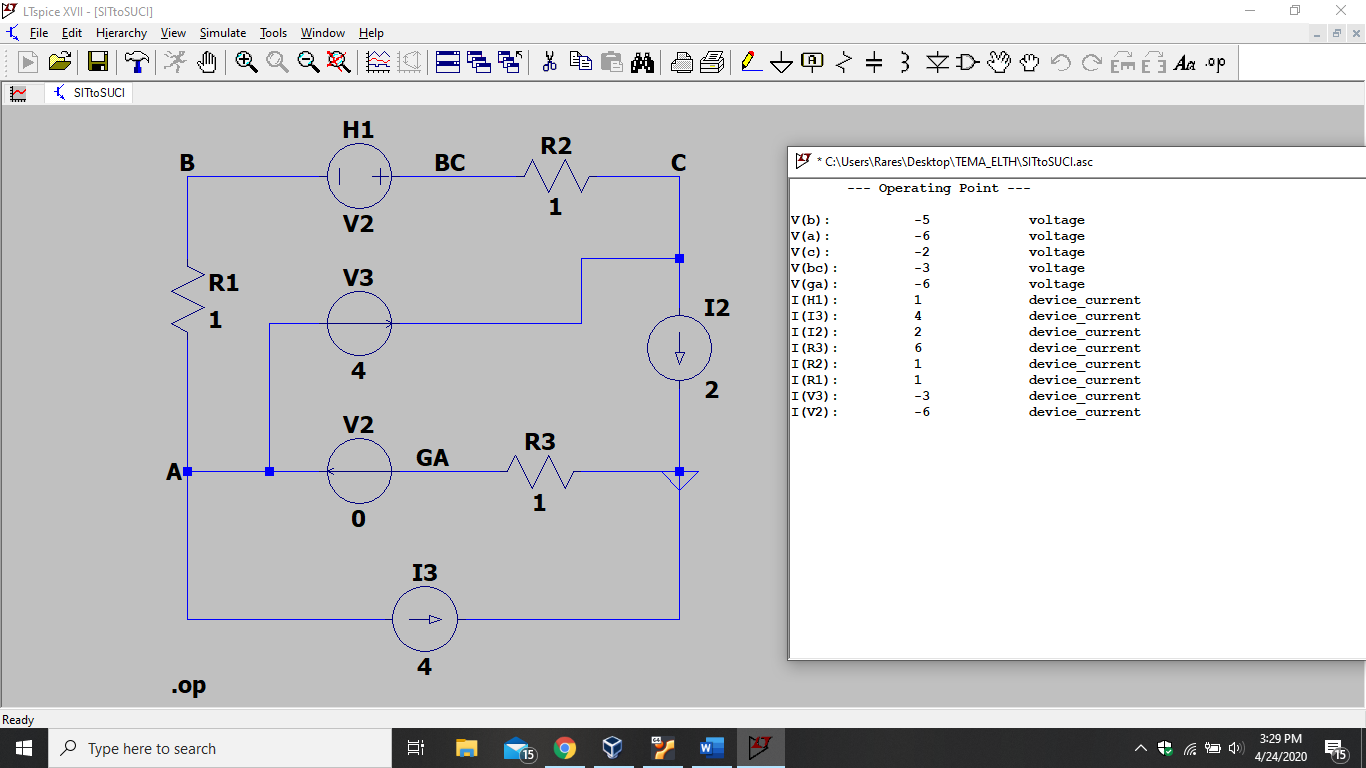
\includegraphics[trim=100 75 100 100,clip,width=\textwidth]{SIT_TO_SUCI}.
	\end{figure}
	\begin{figure}[h!b]
	\begin{center}
	\end{center}
		\vspace{-1.1cm}
		\caption{Reprezentarea cirucitului din Fig. \ref{fig: SUCI} in LTspice.}\label{fig:SIT_TO_SUCI}
	\end{figure}		
			
	\subsection{Transformare SIC \^{i}n SICU}
	\vspace{-0.3cm}
			
	\begin{figure}[H]
	\centering
	\begin{circuitikz}[american]
				
		\draw node[above left= 0.01cm]{A}(0, 0) to [R, l = 1<\ohm>, *-*](0,4) % R1
		(2, 4) to [V, l_ = 2<\volt>] (0, 4) % V2
		(2, 4) to [R, l = 1<\ohm>] (4, 4)node[above right= 0.01cm]{C} % R2
		(4, 4) to [I, l = 2<\ampere>, *-*] (4, 0) % J1
		(4, 0)to [R, l=1<\ohm>] (0, 0) % R3
		%(0, 0) to [V, l_=1<\volt>](2, 0) % V3
		(0, 0) -- (0, -2) to [cI, l_=$1\cdot(V_{C} - V_{A})$, color=red, red](4, -2) -- (4, 0) % J2
		
		(4, 4) -- (3, 3) to [V, l = 4<\volt>] (1, 1) -- (0, 0) %V2	
		;
		
	\end{circuitikz}
	\caption{Circuit generat prin \^{i}nlocuirea SIC cu SICU.}\label{fig: SICU} 
	\end{figure}
	\begin{flushleft}
	\tab Conductan\c{t}a de transfer este egal\u{a} cu 1, iar din Fig. \ref{fig: SIC_TO_SICU}, se observ\u{a} echivalen\c{t}a cu grafurile de curent \c{s}i tensiune reprezentate \^{i}n Fig. \ref{fig: gdc}, respectiv Fig. \ref{fig: gdu}.
	\end{flushleft}
	\begin{figure}[h!b]
	\begin{center}
	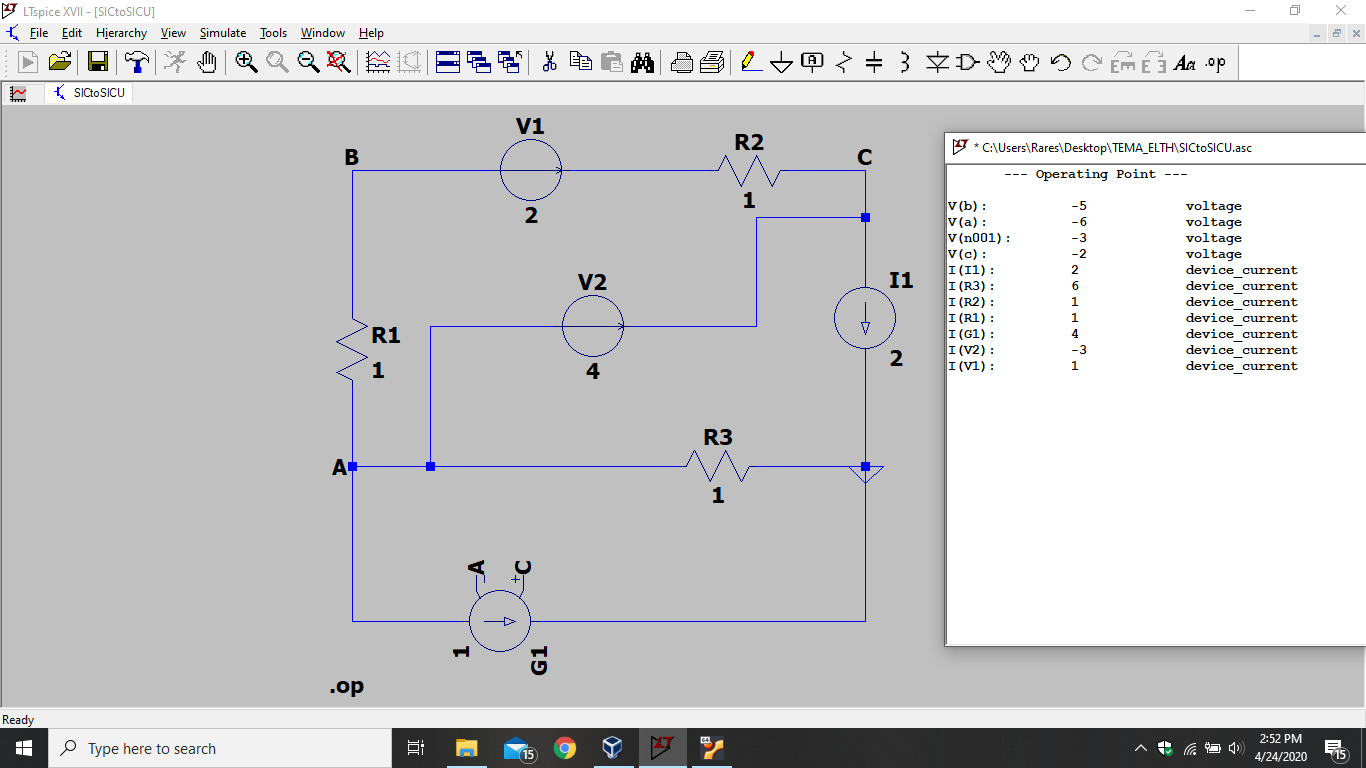
\includegraphics[trim=100 75 100 100,clip,width=\textwidth]{SIC_TO_SICU}
	\end{center}
	\caption{Reprezentarea circuitului din Fig. \ref{fig: SICU} in LTspice.}\label{fig: SIC_TO_SICU}
	\end{figure}

	\pagebreak

	\subsection{Netlists}
	
	\begin{figure}[H]
	\begin{minipage}{0.5\textwidth}
	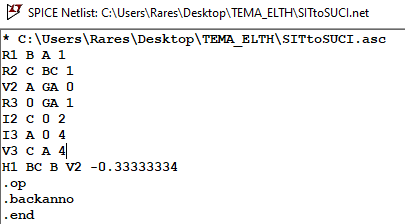
\includegraphics[scale=0.7]{NETLIST_SIT_TO_SUCI}
	\end{minipage}	
	\begin{minipage}{0.5\textwidth}
	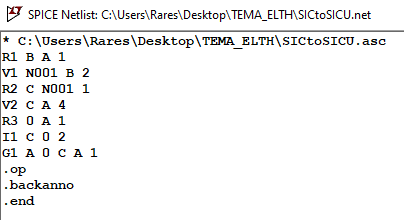
\includegraphics[scale=0.7]{NETLIST_SIC_TO_SICU}	
	\end{minipage}
	\caption{Netlisturile pentru simul\u{a}rile din Fig. \ref{fig:SIT_TO_SUCI} (\^{i}n st\^{a}nga) \c{s}i din Fig. \ref{fig: SIC_TO_SICU} (\^{i}n dreapta)}\label{fig: NETLISTS}
	\end{figure}
\pagebreak
\section{Redactare Latex}
\tab \^{I}n redactarea temei, am folosit \LaTeX. Adaug mai jos c\^{a}teva capturi de ecran ale codului:
	\vspace{0.5cm}

	\hspace{-0.5cm}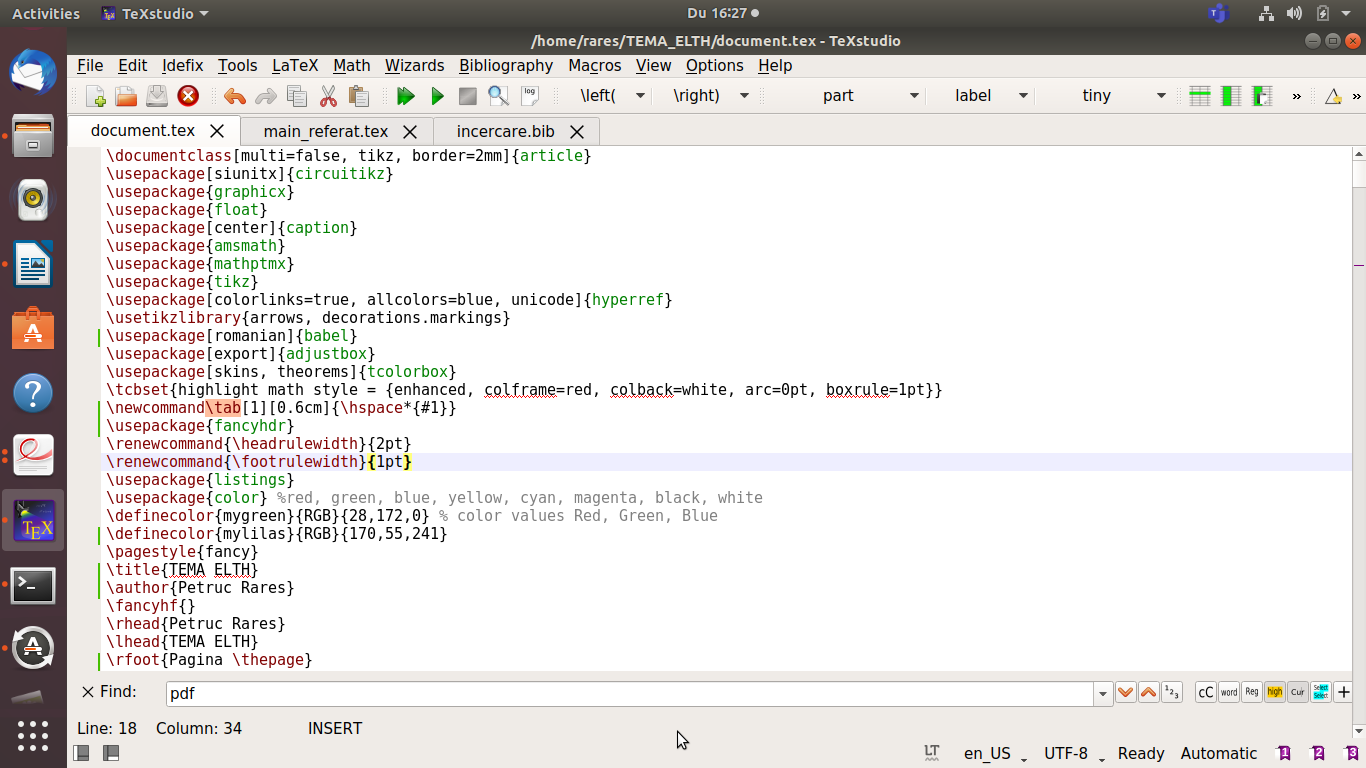
\includegraphics[max width=1.2\textwidth]{PreambulCod}
	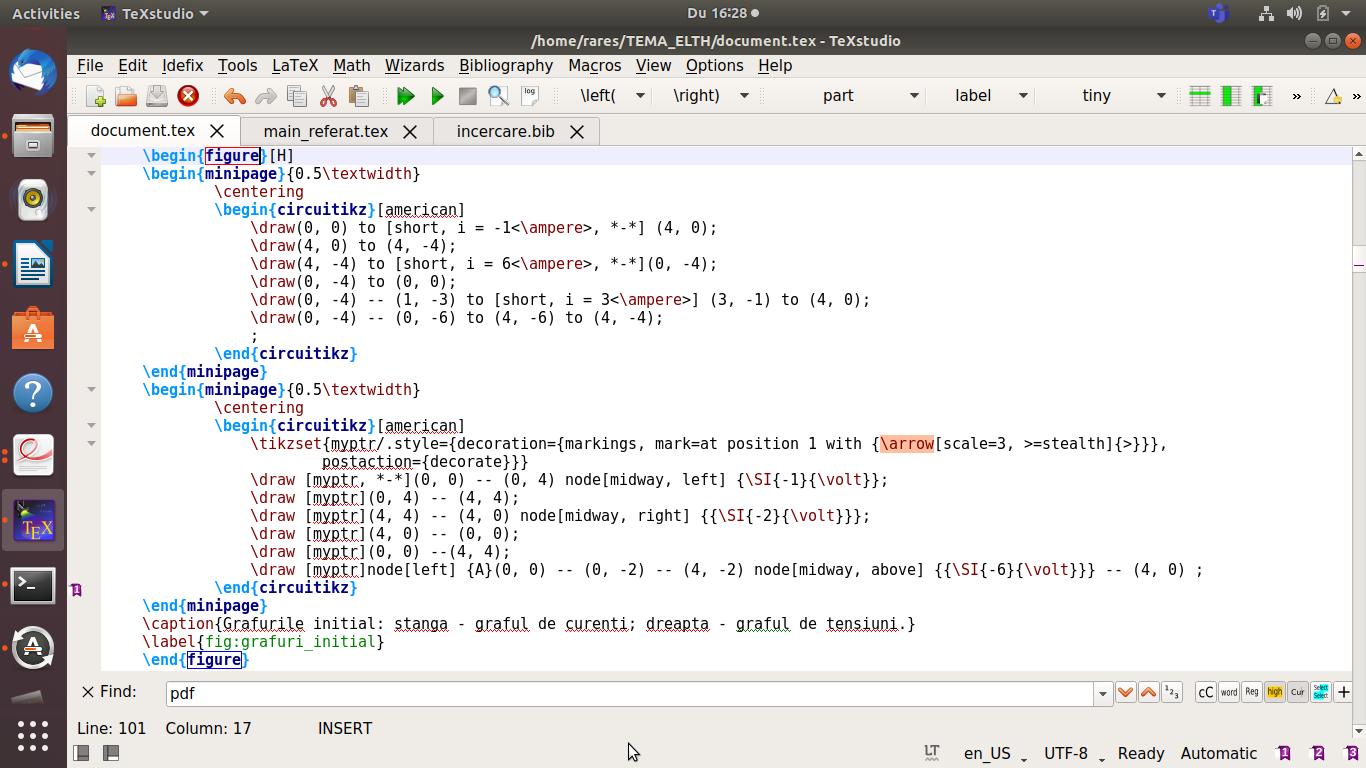
\includegraphics[max width=1.2\textwidth]{COD_Grafuri_intiale}
	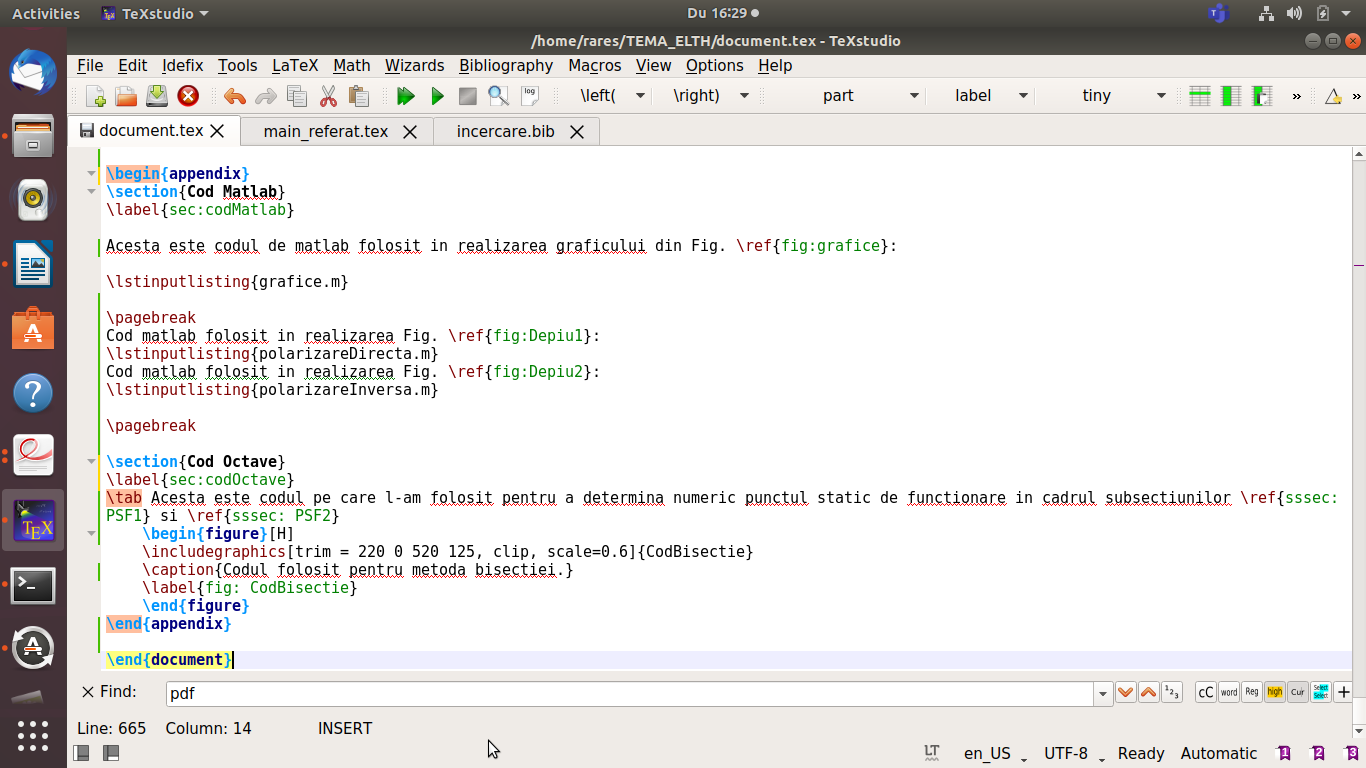
\includegraphics[max width=1.2\textwidth]{COD_FINAL}
\section{Concluzii}
	\tab A fost o tema frumoas\u{a}, care ne-a trecut printr-o mic\u{a} parte din materia studiat\u{a}. Faptul c\u{a} de aceast\u{a} dat\u{a} a trebuit ca noi s\u{a} gener\u{a}m un circuit \c{s}i s\u{a} facem tot ce s-a facut la seminar pe circuitul nostru a fost foarte interesant. \^{I}n opinia mea, redactarea in Latex este o idee foarte bun\u{a}, \^{i}ntrucat se pot realiza lucruri foarte diferite fat\u{a} de alte preparatoare de documente, prin multitudinea pachetelor puse la dispozi\c{t}ia utilizatorului \c{s}i personal, nu am \^{i}nt\^{a}mpinat probleme mari \^{i}n redactarea documentului.
\pagebreak

\addcontentsline{toc}{section}{Bibliografie}
\begin{thebibliography}{99}
	\bibitem{bib:one_article}
	Gabriela Ciuprina, Daniel Ioan, Mihai Popescu, Sorin Lup, Ruxandra B\u{a}rbulescu, Electrotehnica - Breviar de Seminar, Document actualizat la 23 aprilie 2020.
	\bibitem{bib:one_article} Template latex v4
	\bibitem{bib:one_article}
	{\href{https://tex.stackexchange.com/questions/75116/what-can-i-use-to-typeset-matlab-code-in-my-document}{https://tex.stackexchange.com/questions/75116/what-can-i-use-to-typeset-matlab-code-in-my-document}}
		\bibitem{bib:one_article}
	{\href{https://tex.stackexchange.com/questions/122945/coloured-shadowed-boxes-around-equations/122952}{https://tex.stackexchange.com/questions/122945/coloured-shadowed-boxes-around-equations/122952}}
		\bibitem{bib:one_article}
	{\href{https://tex.stackexchange.com/}{https://tex.stackexchange.com/}}
		\bibitem{bib:one_article}
	{\href{https://www.overleaf.com/}{https://www.overleaf.com/}}
\end{thebibliography}

\pagebreak
	
\begin{appendix}
\section{Cod Matlab}
\label{sec:codMatlab}

Acesta este codul de matlab folosit \^{i}n realizarea graficului din Fig. \ref{fig:grafice}:

\lstinputlisting{grafice.m}

\pagebreak
Cod matlab folosit \^{i}n realizarea Fig. \ref{fig:Depiu1}:
\lstinputlisting{polarizareDirecta.m}
Cod matlab folosit \^{i}n realizarea Fig. \ref{fig:Depiu2}:
\lstinputlisting{polarizareInversa.m}

\pagebreak

\section{Cod Octave}
\label{sec:codOctave}
\tab Acesta este codul pe care l-am folosit pentru a determina numeric punctul static de func\c{t}ionare \^{i}n cadrul subsec\c{t}iunilor \ref{sssec: PSF1} si \ref{sssec: PSF2}
	\begin{figure}[H]
	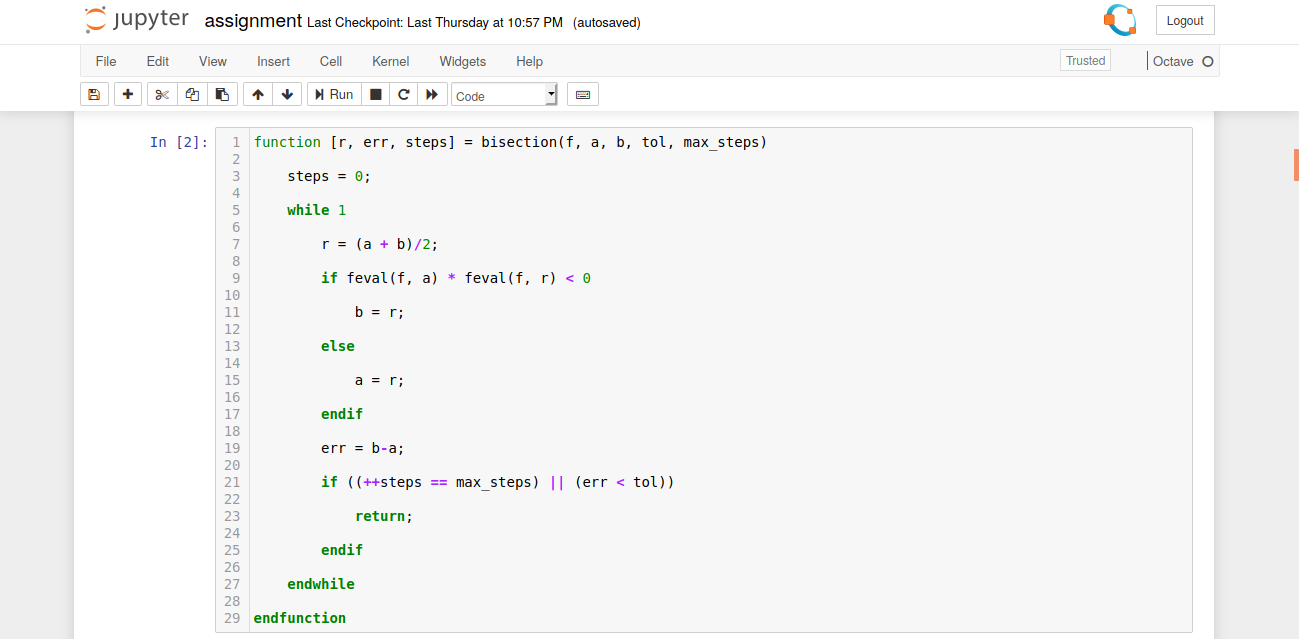
\includegraphics[trim = 220 0 520 125, clip, scale=0.6]{CodBisectie}
	\caption{Codul folosit pentru metoda bisec\c{t}iei.}
	\label{fig: CodBisectie}
	\end{figure}
\end{appendix}

\end{document}